
\title{Tidy Data Neatly Resolves Mass-Spectrometry's Ragged Arrays}
\author{by William Kumler and Anitra E. Ingalls}

\maketitle

\abstract{
Mass spectrometry (MS) is a powerful tool for measuring biomolecules, but the data produced is often difficult to handle computationally because it is stored as a ragged array. In R, this format is typically encoded in complex S4 objects built around environments, requiring an extensive background in R to perform even simple tasks. However, the adoption of tidy data \citep{wickham2014} provides an alternate data structure that is highly intuitive and works neatly with base R functions and common packages, as well as other programming languages. Here, we discuss the current state of R-based MS data processing, the convenience and challenges of integrating tidy data techniques into MS data processing, and present \CRANpkg{RaMS}, a package that produces tidy representations of MS data.
}

\section{Introduction}

Mass-spectrometry (MS) is a powerful tool for identifying and quantifying molecules in laboratory and environmental samples. It has grown enormously over recent decades and has been responsible for countless advances in chemical and biological fields. It is often paired with liquid chromatography (LC) to separate compounds by retention time and improve detection limits. The large quantity of data produced by increasingly rapid and sensitive instruments has facilitated the adoption of computational methods that use algorithms to detect, identify, and quantify molecular signatures.

Many mass-spectrometrists have some exposure to programming, often in R, and this familiarity is expected to increase in the future as computational methods continue to become more popular and available. However, these researchers typically focus on results and the conclusions that can be drawn from them rather than the arcane details of any particular language or package. This produces a demand for simple data formats that can be quickly and easily understood by even a novice programmer. One such representation is the "tidy" data format, which is rapidly growing in popularity among R users for its consistent syntax and large library of supporting packages \citep{wickham2014}. By formatting MS data tidily, the barrier to entry for novice programmers is dramatically reduced, as \CRANpkg{tidyverse} functions learned elsewhere will function identically on MS data.

This article begins by reviewing the current theory and implementation of MS data handling, as driven by three major questions. First, why is it difficult to access and interpret MS data? Second, why should it be easier to do this? Finally, why don't current algorithms make it trivial to do this? In the latter portion of this article, we introduce a new package, called R-based access to Mass Spectrometry data (\pkg{RaMS}) that provides tidy access to MS data and will facilitate future analysis and visualization.

\section{Why is it difficult to access mass-spectrometry data?}

Mass spectrometers produce data in the form of ragged (also sometimes called "jagged") arrays. These data structures contain an unequal number of columns per row because any number of ion masses (\emph{m/z} ratios) may be observed at a given time point. This data is typically managed in a list-of-lists format, with a list of time points each containing a list of the ions observed and their abundances. While this is an effective way to preserve the data structure as it was produced by the instrument, it is less helpful when performing analysis. Typically, analysis (both manual and computational) iterates over \emph{m/z} windows rather than time. The main focus is the extracted ion chromatogram (EIC) which represents all time points for a given mass, and the spectrum of masses obtained at a given time point is less useful during the preliminary review and initial discovery phases. This nested syntax, often itself contained within S4 objects and encoded as an environment, makes it difficult to extract EICs quickly and intuitively.

Even so, "difficult" is a relative assessment. Veteran R programmers have little difficulty writing elegant code that embraces these ragged arrays and the list-of-lists syntax. Indeed, the dominant MS processing package in R, \BIOpkg{MSnbase} currently uses the S4 object system to great effect. However, MS experts are rarely also R experts and have a working familiarity with R rather than a comprehensive background in computer science. This working knowledge typically includes creating plots, subsetting data, and manipulating simple objects but does not extend to the nuances of the S4 object system or methods for rewriting package code. Thus, a package capable of converting these complex data structures into a familiar format appears to be very much in demand.

Finally, it should be noted that existing MS data processing packages are designed to be holistic pipelines which accept raw data and output definitive results. There is very little room for a user's customization beyond the provided function arguments despite the enormous variability in MS setups, usage, and data quality. It is often challenging to access intermediate objects as a way to debug unexpected results, and published code is rarely easy to edit safely due to poor documentation and unit test coverage. These issues are compounded by the agglomerative nature of R packages that build extensively upon other R packages; the popular \BIOpkg{xcms} processing package has over a hundred dependencies installed from across CRAN and Bioconductor, with further functionality provided by unregulated code from GitHub and SourceForge. When combined with additional issues from C++ compilers, versioning, and operating system discrepancies, MS data analysis becomes very much a "black box" with functioning pipelines treated as fragile rather than simple, robust, and reproducible.

\section{Why should it be easier to access mass-spectrometry data?}

Mass-spectrometry data is fundamentally simple. In LC-MS full-scan mode, each data point has three coordinates corresponding to the time, molecular mass, and intensity dimensions. Even the more complex fragmentation data requires only a single additional dimension, fragment mass. While this ignores the large quantity of critical metadata associated with each file that must also be stored somewhere, a core part of MS research is driven by the data alone. In this preliminary stage of analysis, metadata is less relevant than simple exploratory questions about which molecules can be detected and preliminary assessments of data quality. This exploratory phase is driven by rapid, ad hoc discovery and hypothesis testing that typically requires visualizing chromatograms and the raw data to assess quality: this appears to be one of the reasons why R and its built-in plotting ability is so popular for MS analysis \citep{gatto2015}. These queries should be trivial to implement, even for beginning R users, but current data storage methods make them difficult and often time-consuming. Currently, the easiest questions to answer about MS data are metadata-based queries about the instrument that the analyst is usually already able to answer. This is an artifact of information storage in most raw data files, with metadata available readily at the top level and measurements buried deep within.

Raw MS data is typically converted from vendor-specific formats into open-source versions that can be parsed without proprietary software. The modern standard is the mzML document, which has been designed to combine the best aspects of precursor standards in a single universal format \citep{deutsch2010}. These XML documents have well-defined schema built around a controlled vocabulary to enable consistent parsing. Most critically, the development of the modern mzML format established accession numbers for each attribute which (according to the specification document) should never change. This stability means that the data can be accessed robustly with any XML parser. Older formats, such as mzXML, are currently deprecated and will not undergo further development, making them equally stable.

Finally, simple data formats make it easier to work within existing frameworks rather than developing exclusive functions. Tidy data interacts neatly with the entire \pkg{tidyverse} thanks to its shared design philosophy and it's simple to upgrade basic data frames to \CRANpkg{data.table}s for improved access speed. More crucially, however, simple formats make it possible to port MS data to other languages and interfaces. It is straightforward to convert an R data frame to Python's pandas version via the \CRANpkg{reticulate} package, encode it as a SQL database, or export it as a CSV file to be viewed in Excel or other familiar GUIs. The same cannot be said for R's environments and S4 objects. This connectivity ensures that the best tools possible can be applied to a problem, rather than the subset available in a given package or programming language. Simplifying access to and working storage of MS data is a critical step for the further development of fast, accurate algorithms for the detection and quantification of molecules across many areas of science.

\section{Why isn't it already easier to access mass-spectrometry data?}

Of course, there are challenges that make simplification difficult and a trade-off must be made between speed, storage, and sanity. Tidy data favors code readability and intuitiveness over computational efficiency: for example, a list-of-lists model is more memory efficient than the proposed rectangular data structure because each time point is stored once rather than repeated in each row. When multiple files are analyzed simultaneously, tidy data also requires that the filename be repeated similarly, resulting in essentially a doubling of object size in the computer memory. Given that most MS experiments involve tens or hundreds of large files, this is a major concern and current packages handle memory carefully, either reading from disk only what is needed or running files in batches. There are several ways to resolve this problem within the tidy data model as well. During the exploration phase, it is rarely necessary to load all data from files simultaneously, but viewing some portion of the data is still critically important for quality control. With the tidy model, it's not required to import all the data in a single comprehensive step. Instead, quality control files or pooled samples can be viewed as representative of the whole run and rarely challenge memory requirements. Additionally, tidy data makes it easy to subset only the masses of interest for targeted analyses, and the remainder of the data can be discarded from memory. For the final comprehensive analysis, it is much simpler to encode MS data into an external database for access via SQL or other query language when formatted tidily than it is to wrangle current implementations into some accessible object that can handle project sizes larger than the computer's memory.

Theoretically, the ideal data structure for MS data processing speed would invert the current list-of-lists schema by constructing a list of unique \emph{m/z} values, each containing the time points at which that mass ratio was observed and the corresponding intensity. However, this method is complicated by the instrumental error inherent in measuring molecular masses. The same molecule may be measured to have a slightly different mass at each time point, and "binning" these masses together across all time points for a single consensus value risks incorporating nearby masses together even at hypothetical sub-ppm mass accuracy \citep{kind2006}. Instead, \emph{m/z} values are continuous rather than discrete, making it difficult to encode the data in this way. A tidy framework resolves part of this issue by storing the time and \emph{m/z} values in columns that can be indexed by a binary search, such as the one implemented by \pkg{data.table}. This allows for rapid subsetting by both time and \emph{m/z}. Finally, it is worth noting that computers have rapidly grown faster and larger while human intuition has not grown as quickly. This indicates that concerns with processing time and memory will lessen over time and that in the long run, sanity should be prioritized over speed and storage.

There are other reasons that a tidy approach has not yet been implemented for MS data. MS files include large amounts of metadata which should not be discarded, but are challenging to encode efficiently in a rectangular format. A proper tidy approach requires that a separate table be constructed to hold this per-file metadata, with a key such as file name that permits joining the metadata back to the original information. Compared to the monolithic S4 objects constructed by traditional workflows, managing multiple tables may be unappealing. S4 objects also excel at recording each process that is performed on the data, and a specific "processes" slot is found in some objects to record exactly this. However, with the emergence of code sharing and open-source projects it becomes less critical that the data itself records the process because the source code is available.

Finally, a significant history exists for today's methods. \pkg{MSnbase}, the first widely-used R package designed to process MS data, implemented S4 objects as a way to hold entire MS experiments in memory, and dependent packages extend this MSnExp object in various ways rather than discarding it entirely. This development history and connected network of packages is incredibly useful and represents an extensive process of innovation and refinement. We would like to emphasize that the concerns raised here and the package introduced below are not designed to critique or replace this significant effort. Instead, our goal is to function alongside prior work as a way to enable rapid, interactive, and preliminary exploration. Following initial investigation, we recommend using the existing pipelines and extensive package network to establish a reproducible, scripted process of MS data analysis.

\section{The RaMS package}

The \pkg{RaMS} package implements in R a set of methods used to parse open-source mass-spectrometry documents into the R-friendly data frame format. Functions in the package accept file names and the type of data requested as arguments and return rectangular data objects stored in R's memory. This data can then be processed and visualized immediately using base R functions such as plot and subset, passed to additional packages such as \CRANpkg{ggplot2} and \pkg{data.table}, or exported to language-agnostic formats such as CSV files or SQL databases.

\subsection{Installation}

The \pkg{RaMS} package can be installed in two ways:

The release version from CRAN:

\begin{example}
    install.packages("RaMS")
\end{example}

Or the development version from GitHub:

\begin{example}
    # install.packages("remotes")
    remotes::install_github("wkumler/RaMS")
\end{example}

\subsection{Input arguments}

\pkg{RaMS} is simple and intuitive, requiring the memorization of a single new function \code{grabMSdata} with the following usage:

\begin{example}
    grabMSdata(files)
\end{example}

Where \code{files} is a vector of file paths to mzML or mzXML documents, which can be located on the user's computer, a network drive, FTP site, or even at a URL on the Internet. 
Further parameters are documented below in Table \ref{tab:params}:

\begin{table}[h]
    \centering
    \begin{tabularx}{\textwidth}{ l X }
        \toprule
        Parameter & Description \\
        \midrule
        \code{grab\_what} & Specifies the information to extract from the mzML or mzXML file. Can currently accept any combination of "MS1", "MS2", "EIC", "EIC\_MS2", "metadata", and "everything" (the default). \\
        \code{verbosity} & Controls progress messages sent to the console at three different levels: no output, loading bar and total time elapsed, and detailed timing information for each file. \\
        \code{mz} & Used when \code{grab\_what} includes "EIC" or "EIC\_MS2". This argument should be a vector of the \emph{m/z} ratios interesting to the user, if the whole file is too large to load into memory at once or only a few masses are of interest. \\
        \code{ppm} & Used alongside the \code{mz} argument to provide a parts-per-million error window associated with the instrument on which the data was collected. \\
        \code{rtrange} & A length-two numeric vector with start and end times of interest. Often only a subset of the LC run is of interest, and providing this argument limits the data extracted to those between the provided bounds. \\
        \bottomrule
    \end{tabularx}
    \caption{Parameters accepted by the \code{grabMSdata} function.}
    \label{tab:params}
\end{table}

\subsection{Usage}

Extracting data with \code{grabMSdata} returns a list of tables, each named after one of the parameters requested. A \code{grab\_what} argument of \code{"MS1"} will return a list with a single entry, the MS$^1$ (i.e. full-scan data) for all of the files:

\begin{example}
    msfile <- system.file("extdata", "LB12HL_AB.mzML.gz", package = "RaMS")
    msdata <- grabMSdata(files = msfile, grab_what="MS1")
    head(msdata$MS1)
\end{example}

\begin{table}[h]
    \centering
    \begin{tabular}{r|r|r|l}
        \hline
        rt & mz & int & filename\\
        \hline
        4.009 & 104.0710 & 1297755.000 & LB12HL\_AB.mzML.gz\\
        \hline
        4.009 & 104.1075 & 140668.125 & LB12HL\_AB.mzML.gz\\
        \hline
        4.009 & 112.0509 & 67452.859 & LB12HL\_AB.mzML.gz\\
        \hline
        4.009 & 116.0708 & 114022.531 & LB12HL\_AB.mzML.gz\\
        \hline
        4.009 & 118.0865 & 11141859.000 & LB12HL\_AB.mzML.gz\\
        \hline
        4.009 & 119.0837 & 9636.127 & LB12HL\_AB.mzML.gz\\
        \hline
    \end{tabular}
    \caption{Tidy format of RaMS output showing columns of MS$^1$ data, with columns for retention time (rt), mass-to-charge ratio (mz), intensity (int) and name of the source file (filename). Note that this is a subset - the actual object contains 8,500 entries.}
    \label{tab:MS1demo}
\end{table}

This table is already tidied, ready to be processed and visualized with common base R or \pkg{tidyverse} operations. For example, it's often useful to view the maximum intensity observed at each time point: this is known as a base peak chromatogram or BPC. Below are two examples of calculating and plotting a BPC using base R and the \pkg{tidyverse}.

\begin{example}
    # Base R
    BPC <- tapply(msdata$MS1$int, msdata$MS1$rt, max)
    plot(names(BPC), BPC, type="l")
\end{example}

\begin{figure}[ht]
    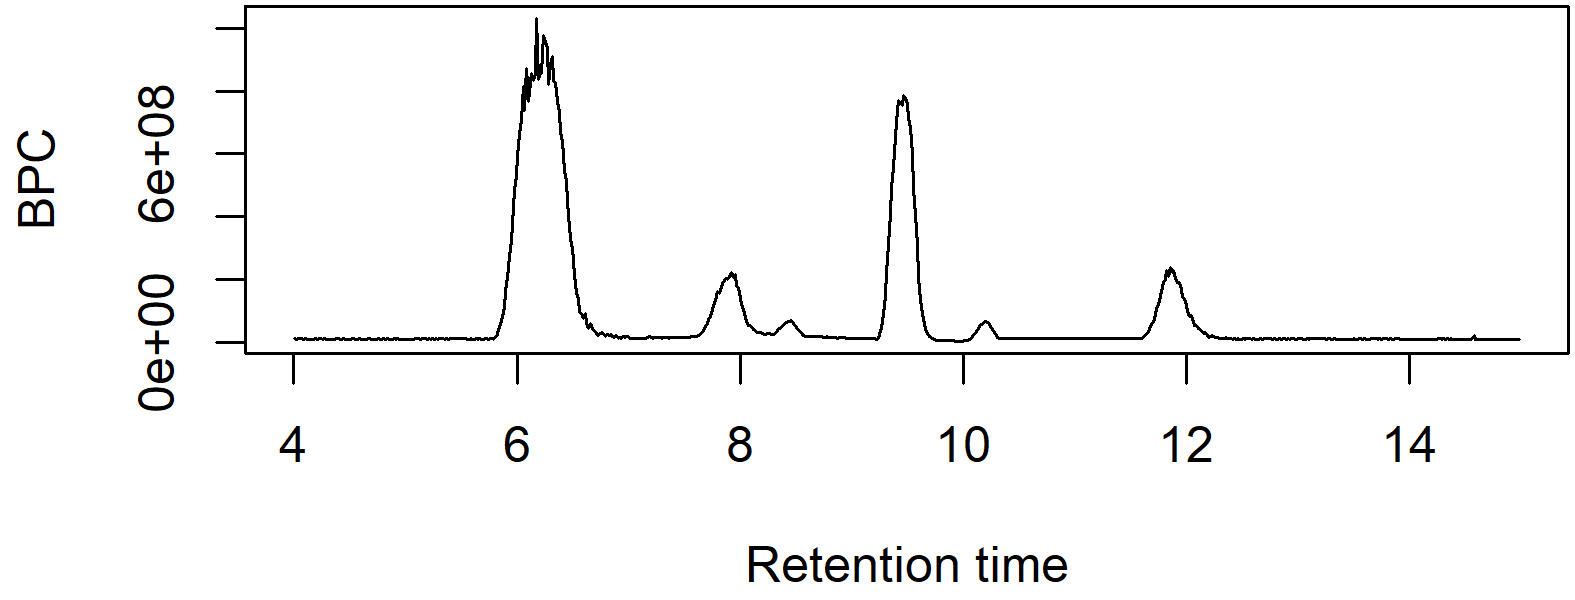
\includegraphics[]{baseRchrom.png}
    \caption{A simple chromatogram plotted using base R. This plot shows the retention time of all compounds in a sample plotted against the maximum intensity at each timepoint. Base graphics were used so the plot is fully customizable with normal graphics options.}
    \label{fig:baseRchrom}
\end{figure}

\begin{example}
    # Tidyverse
    library(tidyverse)
    BPC <- msdata$MS1 %>% 
        group_by(rt) %>% 
        summarize(BPC_int=max(int))
    ggplot(BPC) + geom_line(aes(x=rt, y=BPC_int))
\end{example}

\begin{figure}[h!]
    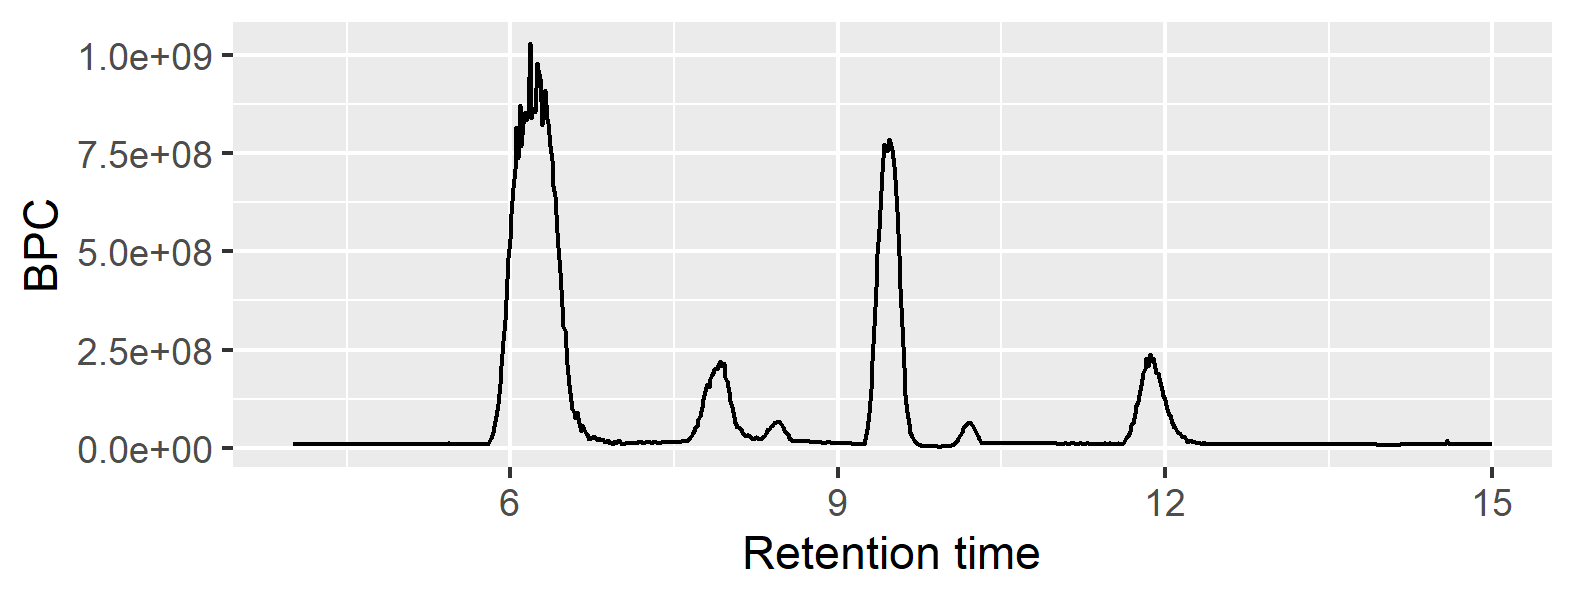
\includegraphics[]{ggplotchrom.png}
    \caption{A simple chromatogram plotted using the \pkg{ggplot2} package. This plot shows the same data as Figure \ref{fig:baseRchrom} of retention time by maximum intensity across compounds but uses \pkg{ggplot2} syntax and defaults.}
    \label{fig:ggplotchrom}
\end{figure}

Importantly, note that the creation of these plots required no special knowledge of the S3 or S4 systems and the plots themselves are completely customizable. While similar packages provide methods for plotting output, it is rarely obvious what exactly is being plotted and how to customize those plots because the data is stored in environments and accessed with custom code. \pkg{RaMS} was written with the beginning R user in mind, and its design philosophy attempts to preserve the most intuitive code possible.

\pkg{RaMS} uses \pkg{data.table} internally to enhance speed, but this also allows for more intuitive subsetting in mass-spectrometry data. With \pkg{data.table}, operations are nearly as easy to write in R as they are to write in natural language, leveraging the user's intuition and decreasing the barrier to entry for non-coder MS experts. For example, a typical request for MS data might be written in natural language as:

\begin{quote}
    "All MS$^1$ data points with \emph{m/z} values between an upper and lower bound, from start time to end time."
\end{quote}

This request can be written in R almost verbatim thanks to \pkg{data.table}'s intuitive indexing and \code{\%between\%} function:

\begin{example}
    msdata$MS1[mz %between% c(upper_bound, lower_bound) & 
        rt %between% c(start_time, end_time)]
\end{example}

Most importantly, this syntax doesn't require the mass-spectrometrist to have an understanding of how the data is stored internally. Current implementations use S4 objects with slots such as "chromatograms" and "spectra" or derivatives of these, despite their inconsistent usage across the field and unclear internal structure. \citep{smith2015}

\pkg{RaMS} enhances the intuitive nature of \pkg{data.table}'s requests slightly by providing the pmppm function, short for "plus or minus parts-per-million (ppm)". Masses measured on a mass-spectrometer have a certain degree of inherent deviation from the true mass of a molecule, and the size of this error is a fundamental property of the instrument used. This means that mass-spectrometrists are often interested in not only the data points at an exact mass, but also those within the ppm error range. MS data exploration often makes requests for data in natural language like:

\begin{quote}
    "All MS$^1$ data points with \emph{m/z} values within the instrument's ppm error of a certain molecule's mass"
\end{quote}

Which can again be expressed in R quite simply as:

\begin{example}
    msdata$MS1[mz %between% pmppm(molecule_mass, ppm_error)]
\end{example}

\subsection{Internals}

Fundamentally, \pkg{RaMS} can be considered an XML parser optimized for mzML and mzXML documents. The rigorous specification and detailed documentation make it possible for a generic XML parser to efficiently extract the document data. In R, the \CRANpkg{xml2} package provides modern parsing capabilities and is efficient in both speed and memory usage by calling C's libxml2 library, making it an attractive choice for this processing step. Much of \pkg{RaMS}'s internal code consists of a library of XPath expressions used to access specific nodes and extract the (often compressed) values . Table \ref{tab:XPathparams} below provides several examples of XPath expressions used to extract various parameters from the mzML internals:

\begin{table}[h]
\begin{center}
\begin{tabular}{|c|c|}
    \toprule
    Parameter of interest & mzML XPath expression \\
    \midrule
    Fragmentation level & //spectrum/cvParam[@name="ms level"] \\
    Retention time & //scanList/scan/cvParam[@name="scan start time"] \\
    \emph{m/z} values & //binaryDataArrayList/binaryDataArray[1]/binary \\
    Intensity values & //binaryDataArrayList/binaryDataArray[2]/binary \\
    Polarity (for positive mode) & //spectrum/cvParam[@accession="MS:1000130"] \\
    \bottomrule
\end{tabular}
\end{center}
    \caption{A few example parameters extracted from the mzML file and the corresponding XPath expression used to extract it.}
    \label{tab:XPathparams}
\end{table}

These sample expressions illustrate the controlled vocabulary of the mzML parameters (the cvParam elements above) and the remarkable stability of the specification that permits optimization. While the "polarity" parameter for positive mode is the only one above that is specified via its accession number ("MS:1000130"), it's worth noting that the other parameters also have unique accession number attributes that could be used but instead have been foregone in favor of readability.

MS data files are often highly compressed and the \emph{m/z} and intensity data is typically encoded as base 64 floating point arrays. MS data extracted from the binary data array must then first be decoded from base64 to binary using the \CRANpkg{base64enc} package, then decompressed if necessary using R's base \code{memDecompress} function, and finally cast to double-precision floating point values via base R's \code{readBin}.

After the data has been extracted from the XML document, \pkg{RaMS} uses the \pkg{data.table} package to provide fast aggregation and returns \pkg{data.table} objects to the user. This is also the step which converts the data from a ragged array format into a tidy format, and neatly illustrates the strength of tidy data. Rather than continuing to store the data as a list-of-lists and preserving the nested data structure, this step creates separate columns for retention time (rt) and \emph{m/z} (mz) values. This allows the user to perform rapid binary searches on both the retention time and \emph{m/z} columns and can greatly accelerate the extraction of individual masses of interest, as is often the goal when analyzing MS data.

\subsection{Comparison to similar packages}

While many packages exist to process MS data within R, very few can be found that actually read the raw data into the R environment. The dominant package by far is \pkg{MSnbase}, which describes itself as providing "infrastructure for manipulation, processing and visualisation of mass spectrometry and proteomics data", and is thus very similar to \pkg{RaMS}. \pkg{MSnbase} itself calls the Bioconductor package \BIOpkg{mzR} to provide the C++ backend used to parse the raw XML data. Other packages include \CRANpkg{readMzXmlData} and \CRANpkg{MALDIquantForeign}, both developed by Sebastian Gibb and hosted on CRAN. One additional package to note is the \pkg{caMassClass} package that no longer exists on CRAN but code from which can be found in the \CRANpkg{CorrectOverloadedPeaks} package and only parses the deprecated mzXML format. Finally, the \BIOpkg{Spectra} package is under active development by the RforMassSpectrometry initiative and represents a useful comparison for other cutting-edge frameworks that will be expanded in the future \citep{rainer2022}. However, all of these packages preserve the list-of-list format and none produce naturally tidy representations.

This section illustrates how \pkg{RaMS} compares to \pkg{MSnbase} as the current dominant processing package and \pkg{Spectra} as the next iteration of MS processing. \pkg{MSnbase} has undergone constant revision since its inception in 2010, while \pkg{Spectra} has been under development since 2020. The most recent version of \pkg{MSnbase} as of this writing was announced in 2020 and focuses on the new "on-disk" infrastructure that loads data into memory only when needed. This new infrastructure and the legacy storage mode released in the first version of \pkg{MSnbase} provide useful comparisons for \pkg{RaMS} in terms of memory usage and speed and the \pkg{Spectra} package will provide a useful future-oriented comparison. As noted above, however, \pkg{RaMS} has different goals from either of these packages. \pkg{RaMS} is optimized for raw data visualization and rapid data exploration while \pkg{MSnbase} and \pkg{Spectra} are designed to provide a solid foundation for more streamlined data processing and these packages all can work neatly in concert rather than replacing each other. 

To compare the different methods, ten MS files were chosen from the MassIVE dataset \newline MSV000080030 to mimic the large-experiment processing of \citet{gatto2015}. Methods were compared in terms of memory usage, time required to load the data into R's working memory, and the time required to subset an EIC and plot the data. Due to the differences in method optimization, we expected \pkg{MSnbase} to be significantly faster when loading the data, \pkg{RaMS} to be significantly faster during subsetting and plotting, and \pkg{MSnbase} to have the smallest memory footprint. The \pkg{Spectra} package's capabilities were less well known in advance but should represent a consistent improvement over \pkg{MSnbase}. These expectations were well-validated by the results shown in Figure \ref{fig:speedsizecomp}.

\begin{figure}[ht!]
    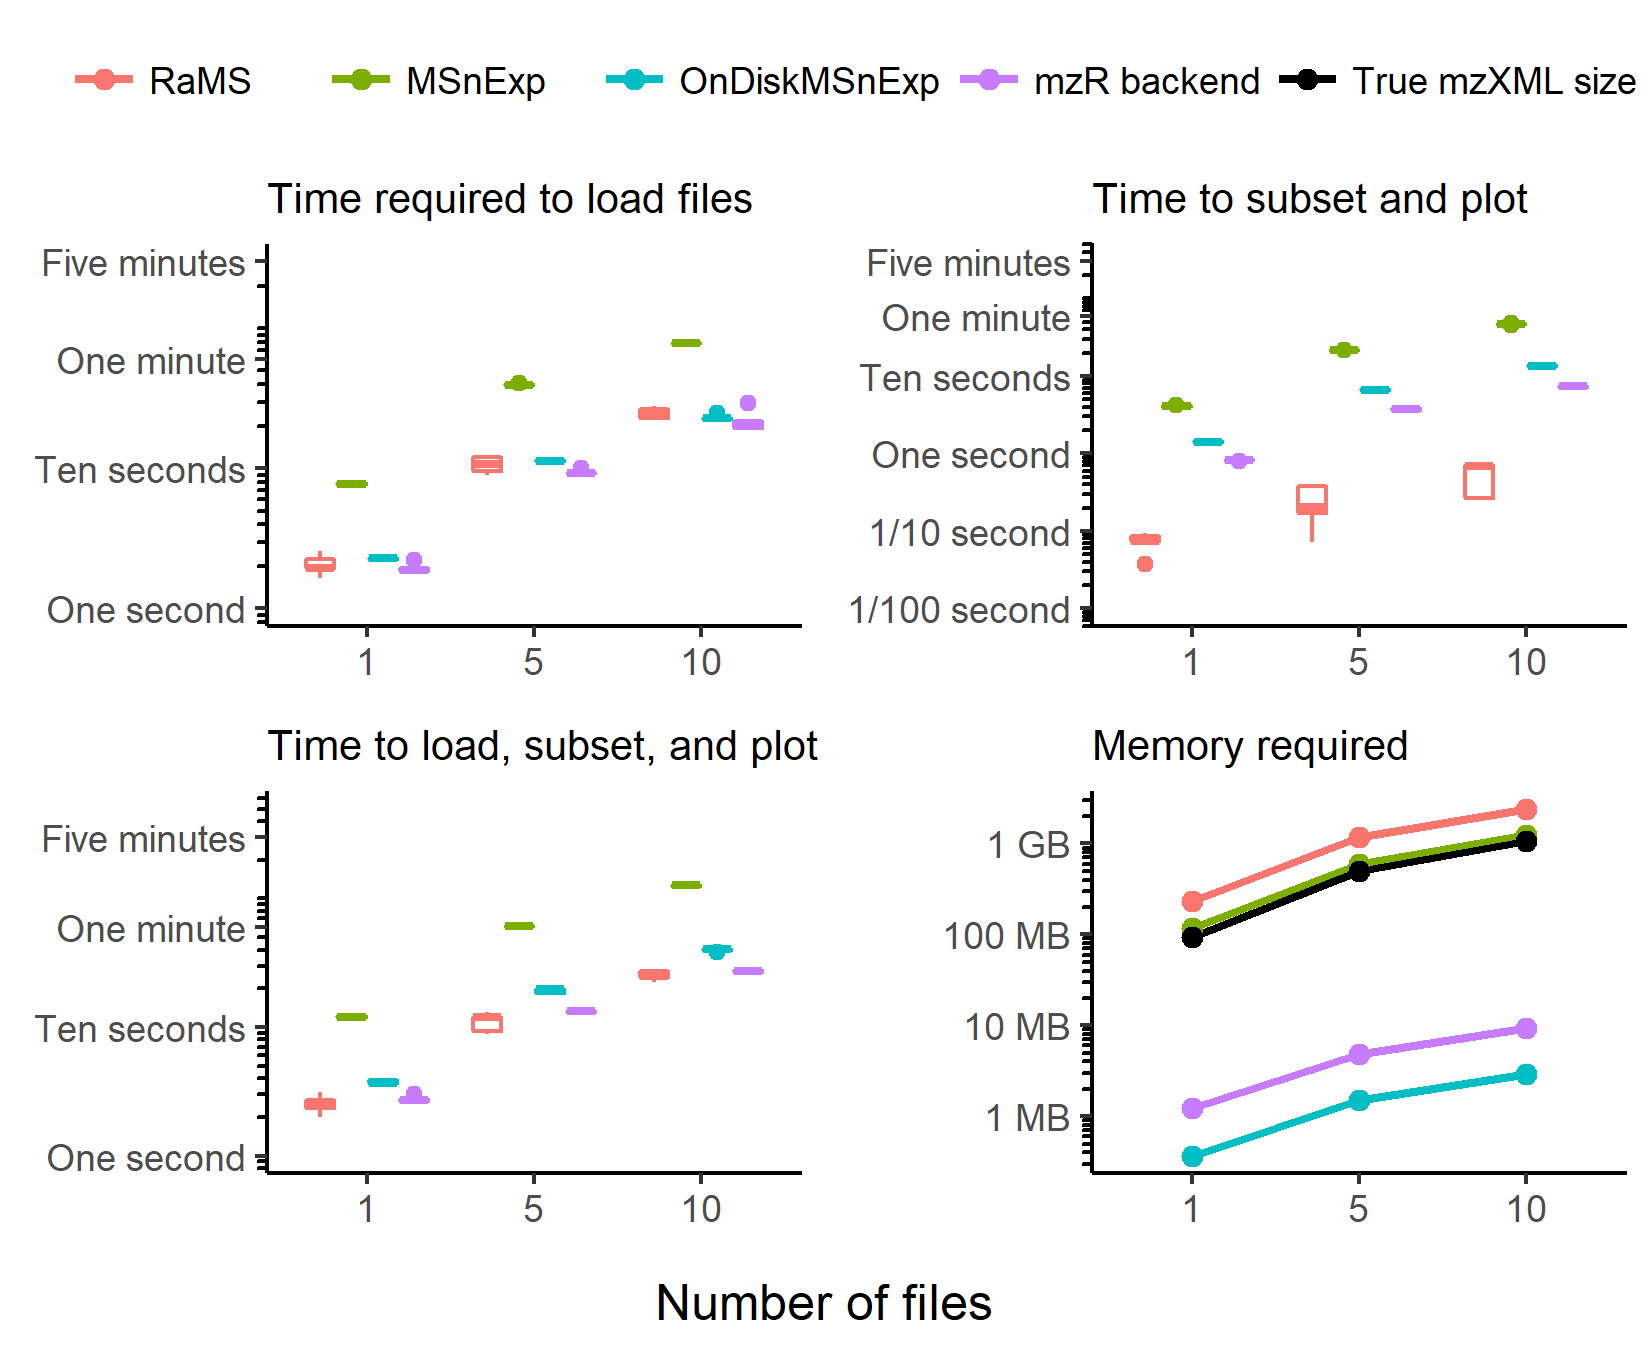
\includegraphics[]{speedsizecomp.png}
    \caption{Time and memory required by \pkg{RaMS} compared to the \pkg{MSnbase} and \pkg{Spectra} methods across 1, 5, and 10 mzXML files. The top-left plot shows the time required to load the mzXMLs into memory (\pkg{RaMS} and \pkg{MSnExp}) or construct pointers (OnDiskMSnExp, \pkg{Spectra}'s mzR backend) with the MSnExp object taking approximately an order of magnitude longer than the other methods. The top-right plot shows the time required to subset the data by \emph{m/z} to a single chromatogram and plot that subset after the object has already been created. The \pkg{RaMS} package performs this approximately an order of magnitude faster than the other packages and the \pkg{Spectra} package is second-fastest, with \pkg{RaMS} taking less than a second for up to 10 mzXMLs and the \pkg{Spectra} package taking between one and ten seconds depending on the number of files to be subset. The bottom-left plot shows a combination of the two plots above by timing each package as it performs the full object construction, subsets to a single chromatogram, and plots it with \pkg{RaMS} again the fastest among the packages. The bottom-right plot shows the memory required for each package across different numbers of files as well as the size of the original mzXML documents as a benchmark. Both \pkg{RaMS} and the MSnExp objects occupied more space in RAM than the original file size (\pkg{RaMS} occuying approximately 2x as much memory, MSnExp closer to 1.1x), while the OnDiskMSnExp and mzR backend were consistently two orders of magnitude smaller. Times were obtained by the \CRANpkg{microbenchmark} package and object sizes were obtained with \CRANpkg{pryr}. Note the log-scaled y-axes.}
    \label{fig:speedsizecomp}
\end{figure}


\pkg{RaMS} performed better than expected on the data load-time metric, taking approximately the same amount of time as the new on-disk \pkg{MSnbase} backend and the \pkg{Spectra} package and significantly less than the old in-memory method. This was surprising because while \pkg{RaMS} is performing the physical I/O process essentially equivalent to the creation of the MSnExp, both the OnDiskMSnExp method and the Spectra object instead create a system of pointers to the data and don't actually read the data into memory. However, the new backend begins to perform better as the number of files increases and proportional improvements are expected with even larger file quantities. The \pkg{Spectra} package, as expected, shows consistent improvements over both \pkg{MSnbase} backends.

For the subsetting and plotting metric, our expectation that \pkg{RaMS} would be the fastest method was validated by times approximately two orders of magnitude smaller than those obtained by \pkg{MSnbase} (note the log scale used in the figure). These results also validated earlier results demonstrating the superiority of the new on-disk method \citep{gatto2015} and the improvements in the new \pkg{Spectra} package. The sub-second subset and plot times of \pkg{RaMS} are so much smaller than the other timings recorded in this trial that \pkg{RaMS} essentially has a single fixed cost associated with the initial data import, making it ideal for the exploratory phase of data analysis where files are loaded once and then multiple chromatograms may be extracted and reviewed. This design also aligns with the user's expected workflow in which data import is accepted as a time-consuming task, but subsequent analysis should be relatively seamless and instantaneous.

The greatly reduced subsetting and plotting time required by \pkg{RaMS} and the observation that file load times and data plotting times were approximately equal for MSnbase led to the creation of the bottom-left graph in Figure \ref{fig:speedsizecomp}. This follow-up analysis highlights that the slightly increased file load time of \pkg{RaMS} combined with the very short subsetting and plotting phase is actually less than the total time required by \pkg{MSnbase} and \pkg{Spectra} to read, subset, and plot, establishing \pkg{RaMS} as the fastest option even if the end goal is to extract a single chromatogram. This follow-up also demonstrates the largest improvements of the new \pkg{MSnbase} on-disk method over the old one and the clearest improvements in \pkg{Spectra}.

As expected, this speed comes at a cost. \pkg{RaMS} has a larger memory footprint than even the old in-memory MSnExp object. While all three objects grew approximately linearly with the number of files processed, the \pkg{RaMS} object was approximately 2 times larger than the in-memory \pkg{MSnbase} object and several orders of magnitude larger than the new, on-disk version. This was expected because \pkg{RaMS} stores retention time and filename information redundantly in the tidy format while the list-of-lists method only stores that information once. In fact, the \pkg{RaMS} object size was larger than the uncompressed mzXML files themselves! However, this trade-off can be minimized through the use of \pkg{RaMS}'s vectorized \code{grab\_what = "EIC"} and \code{grab\_what = "EIC\_MS2"} functions that can extract a vector of masses of interest and discard the remainder of the data to free up memory for analyses where the specific ions of interest are known beforehand. The general lesson from this analysis seems to be that if the memory is available and a quick and intuitive interaction is desired, \pkg{RaMS} is now the top contender. For other purposes, \pkg{MSnbase} or \pkg{Spectra} remain the obvious choices depending on expected workflow.

\subsection{Broader interactions}

\pkg{RaMS} is intentionally simple. By encoding MS data in a rectangular, long data format, \pkg{RaMS} facilitates not only R-specific development but contributes to MS analysis across languages and platforms. At the most basic level, subsets of interest can be exported as CSV files for use in any language that can read this ubiquitous format. Even users with zero programming background are familiar with Excel and other spreadsheet GUIs, so this method of export and data-sharing improves transparency by allowing anyone to open the raw data corresponding to compounds of interest.

The list-of-tables format that \pkg{RaMS} returns was inspired by traditional relational databases, and this provides a slightly more complex method of storing data with several advantages over CSV export. The dominant convenience of relational databases is that they can grow almost indefinitely, rather than being limited by computer memory. While existing packages perform admirably when operating on files that fit into RAM, there are few good solutions for the MS experiments that can exceed hundreds of gigabytes in size. Both batching and subset analysis face issues with systematic inter-sample variation rarely controlled for across subsets. Additionally, an external relational database can be easily appended with additional files as experiments continue to be performed, rather than demanding that all samples be run before any analysis can begin. \pkg{RaMS} output can be easily written to SQL databases using existing packages such as \CRANpkg{DBI} and \CRANpkg{RSQLite}:

\begin{example}
    library(DBI)
    db <- dbConnect(RSQLite::SQLite(), "msdata.sqlite")
    dbWriteTable(db, "MS1", msdata$MS1)
    dbListTables(db)
    dbGetQuery(db, "SELECT * FROM MS1 LIMIT 3")
    dbDisconnect(db)
\end{example}

Finally, with \pkg{reticulate}, R data frames can be directly coerced into Pandas DataFrames. This allows for an unprecedented degree of interaction between R and Python for MS data analysis, reducing the need for parallel development in both languages and allowing the optimal functions to be used at each step rather than the limited selection that have already been implemented in R or Python. As MS data exploration and analysis continues to grow increasingly machine-learning heavy, allowing R to interact elegantly with Python enables the best of R's extensive MS analysis history with Python's powerful interfaces to deep learning frameworks such as TensorFlow and Pytorch.

\section{Summary}

In this paper, we discussed the current paradigm of MS data analysis in R and identify an area where tidy data techniques significantly improve user experience and support increased interaction with other packages and software. We also present \pkg{RaMS} as a package that fills this gap by presenting MS data to the R user in a tidy format that can be instantly queried and plotted.

\section{Acknowledgements}

We are grateful to members of the Ingalls Lab and other labs at the University of Washington who gave invaluable feedback on early versions of this package and the philosophy behind it. Katherine Heal and Laura Carlson generated the data used in the demo files and were early adopters, and Angie Boysen and Josh Sacks provided crucial testing and application of the package. We also thank both anonymous reviewers for their insightful commentary and suggestions that improved both the manuscript and the CRAN package. This work was supported by grants from the Simons Foundation (329108, 385428, and 426570, A.E.I.).  

\bibliography{kumler-ingalls-rams}

\address{William Kumler\\
  University of Washington School of Oceanography\\
  1501 NE Boat St., Seattle, WA 98105\
  United States of America\\
  ORCiD: 0000-0002-5022-8009\\
  \email{wkumler@uw.edu}}
  
\address{Anitra E. Ingalls\\
  University of Washington School of Oceanography\\
  1501 NE Boat St., Seattle, WA 98105\
  United States of America\\
  ORCiD: 0000-0003-1953-7329\\
  \email{aingalls@uw.edu}}
